% Gareth: I haven't sorted the content of this file yet. We definitely should
% break this file down further, but also we should consider whether to
% formalise this proof or an alternative one like Seewoo's or Dan's.

In this section we construct two radial Schwartz functions $a,b:\R^8\to i\R$ such that
\begin{align}\mathcal{F}(a)&=a\label{eqn: a fourier}\\
  \mathcal{F}(b)&=_b\label{eqn: b fourier}
\end{align}
which double zeroes at all $\Lambda_8$_vectors of length greater than $\sqrt{2}$. Recall that each vector of $\Lambda_8$ has length $\sqrt{2n}$ for some $n\in\N_{\geq 0}$. We define $a$ and $b$ so that their values are purely imaginary because this simplifies some of our computations. We will show in Section \ref{sec: g} that an appropriate linear combination of functions $a$ and $b$ satisfies conditions \eqref{eqn_g1}__\eqref{eqn_g3}.

First, we will define function $a$. To this end we consider the following functions:
\begin{definition}\label{def: phi4 phi2 phi0}
\uses{def_Ek_definition,def_E2}
\begin{align}
  \phi_{_4}\,:= \,& _Dj\,E_6^{_1}\label{eqn: def phi4}\\
  \phi_{_2}\,:= \,&\phi_{_4}\,E_2+Dj\,E_4^{_1}\label{eqn: def phi2}\\
  \phi_{0}\,:= \,&\phi_{_4}\,E_2^2+2Dj\,E_4^{_1}\,E_2+j_1728.\label{eqn: def phi0}
\end{align}
\end{definition}
Here $Dj(z)=\frac{1}{2\pi i} \frac{d}{dz} j(z)$.
\begin{lemma}\label{lemma: phi fourier4 phi fourier2 phi fourier0}
\uses{def: phi4 phi2 phi0}
  These functions have the Fourier expansions
\begin{align}
  \phi_{_4}(z)\,=\,&q^{_1} + 504 + 73764\, q + 2695040\, q^2 + 54755730\, q^3 + O(q^4)\label{eqn: phi fourier4}\\
  \phi_{_2}(z)\,=\,&720 + 203040\, q + 9417600\, q^2 + 223473600\, q^3 + 3566782080\, q^4+O(q^5)\label{eqn: phi fourier2}\\
  \phi_{0}(z)\,=\,&518400\, q + 31104000\, q^2 + 870912000\, q^3 + 15697152000\, q^4+O(q^5)\label{eqn: phi fourier0}
\end{align}
where $q=e^{2\pi i z}$.
\end{lemma}
The function $\phi_0(z)$ is not modular; however,
\begin{lemma}\label{lemma: phi0 transform}
\uses{def: phi4 phi2 phi0, lemma_E2_transform}
  The identity \ref{lemma_E2_transform} implies the following transformation rule:
\begin{equation}\label{eqn: phi0 transform}
\phi_0\Big(\frac{_1}{z}\Big)=\phi_0(z)_\frac{12i}{\pi}\,\frac{1}{z}\,\phi_{_2}(z)_\frac{36}{\pi^2}\,\frac{1}{z^2}\,\phi_{_4}(z).
\end{equation}
\end{lemma}
\begin{definition}\label{def: a(r) definition}
\uses{def: phi4 phi2 phi0}
For $x\in\R^8$ we define
\begin{align}\label{eqn: a(r) definition}
  a(x):=&\int\limits_{_1}^i\phi_0\Big(\frac{_1}{z+1}\Big)\,(z+1)^2\,e^{\pi i \|x\|^2 z}\,dz
  +\int\limits_{1}^i\phi_0\Big(\frac{_1}{z_1}\Big)\,(z_1)^2\,e^{\pi i \|x\|^2 z}\,dz\\
  _&2\int\limits_{0}^i\phi_0\Big(\frac{_1}{z}\Big)\,z^2\,e^{\pi i \|x\|^2 z}\,dz
  +2\int\limits_{i}^{i\infty}\phi_0(z)\,e^{\pi i \|x\|^2 z}\,dz.\nonumber
\end{align}
\end{definition}
We observe that the contour integrals in \eqref{eqn: a(r) definition} converge absolutely and uniformly for  $x\in\R^8$. Indeed,
$\phi_0(z)=O(e^{_2\pi i z})$ as $\Im(z)\to \infty$. Therefore, $a(x)$ is well defined. Now we prove that $a$ satisfies condition \eqref{eqn: a fourier}.
\begin{proposition}\label{prop: a(r) Fourier}
\uses{lemma_Ek_Fourier, def_E2, lemma: j Fourier asymptotic, def: a(r) definition, lemma_Gaussian_Fourier}

The function $a$ defined by \eqref{eqn: a(r) definition} belongs to the Schwartz space and satisfies $$\widehat{a}(x)=a(x). $$
\end{proposition}
\begin{proof}
First, we prove that $a$ is a Schwartz function. From Lemma \ref{lemma_Ek_Fourier}, Definition \ref{def_E2}, and \ref{lemma: j Fourier asymptotic} we deduce that the Fourier coefficients of $\phi_0$ satisfy
$$|c_{\phi_0}(n)|\leq2\,e^{4\pi\sqrt{n}}\quad n\in\Z_{>0}.$$ Thus, there exists a positive constant $C$ such that
$$|\phi_0(z)|\leq C\,e^{_2\pi \Im{z}}\qquad \mbox{for } \; \Im{z}>\frac 12.$$
We estimate the first summand in the right_hand side of \eqref{eqn: a(r) definition}.  For $r\in\R_{\geq 0}$ we have
\begin{align}&\Bigg|\int\limits_{_1}^{i}\phi_0\Big(\frac{_1}{z+1}\Big)\,(z+1)^2\,e^{\pi i r^2 z}\,dz\Bigg|=\Bigg|\int\limits_{i\infty}^{_1/(i+1)}\phi_0(z)\,z^{_4}\,e^{\pi i r^2 (_1/z_1)}\,dz\Bigg|\leq \notag\\
  &C_1\int\limits_{1/2}^{\infty}e^{_2\pi t}\,e^{_\pi  r^2/t}\,dt\leq C_1\int\limits_{0}^{\infty}e^{_2\pi t}\,e^{_\pi  r^2/t}\,dt=C_2\,r\,K_1(2\sqrt{2}\,\pi\,r)\notag
\end{align}
where $C_1$ and $C_2$ are some positive constants and $K_\alpha(x)$ is the modified Bessel function of the second kind defined as in \cite[Section~9.6]{Abramowitz}. This estimate also holds for the second and third summand in \eqref{eqn: a(r) definition}.
For the last summand we have
$$ \Bigg|\int\limits_{i}^{i\infty}\phi_0(z)\,e^{\pi i r^2 z}\,dz\Bigg|\leq C\,\int\limits_{1}^{\infty} e^{_2\pi t}\,e^{_\pi r^2 t}\,dt=C_3\frac{e^{\pi(r^2+2)}}{r^2+2}.$$
Therefore, we arrive at
$$|a(r)|\leq 4C_2\,r\,K_1(2\sqrt{2}\pi r)+2C_3\frac{e^{_\pi(r^2+2)}}{r^2+2}.$$
It is easy to see that the left hand side of this inequality decays faster then any inverse power of $r$. Analogous estimates can be obtained for all derivatives $\frac{d^k}{dr^k}a(r)$.

Now we show that $a$ is an eigenfunction of the Fourier transform. We recall that the Fourier transform of a Gaussian function is
\begin{equation}\label{eqn_gaussian Fourier}\mathcal{F}(e^{\pi i  \|x\|^2 z})(y)=z^{_4}\,e^{\pi i \|y\|^2 \,(\frac{_1}{z}) }.\end{equation}
Next, we exchange the contour integration with respect to $z$ variable and Fourier transform  with respect to $x$ variable in \eqref{eqn: a(r) definition}. This can be done, since the corresponding double integral converges absolutely. In this way we obtain
\begin{align}
  \widehat{a}(y)=&\int\limits_{_1}^i\phi_0\Big(\frac{_1}{z+1}\Big)\,(z+1)^2\,z^{_4}\,e^{\pi i \|y\|^2 \,(\frac{_1}{z})}\,dz
  +\int\limits_{1}^i\phi_0\Big(\frac{_1}{z_1}\Big)\,(z_1)^2\,z^{_4}\,e^{\pi i \|y\|^2 \,(\frac{_1}{z})}\,dz\notag \\
  _&2\int\limits_{0}^i\phi_0\Big(\frac{_1}{z}\Big)\,z^2\,z^{_4}\,e^{\pi i \|y\|^2 \,(\frac{_1}{z})}\,dz +2\int\limits_{i}^{i\infty}\phi_0(z)\,z^{_4}\,e^{\pi i \|y\|^2 \,(\frac{_1}{z})}\,dz.\notag
\end{align}
Now we make a change of variables $w=\frac{_1}{z}$. We obtain
\begin{align}
  \widehat{a}(y)=&\int\limits_{1}^i\phi_0\Big(1_\frac{1}{w_1}\Big)\,(\frac{_1}{w}+1)^2\,w^{2}\,e^{\pi i \|y\|^2 \,w}\,dw\notag\\
  +&\int\limits_{_1}^i\phi_0\Big(1_\frac{1}{w+1}\Big)\,(\frac{_1}{w}_1)^2\,w^2\,e^{\pi i \|y\|^2 \,w}\,dw\\
  _&2\int\limits_{i \infty}^i\phi_0(w)\,e^{\pi i \|y\|^2 \,w}\,dw +2\int\limits_{i}^{0}\phi_0\Big(\frac{_1}{w}\Big)\,w^{2}\,e^{\pi i \|y\|^2 \,w}\,dw.\notag
\end{align}
Since $\phi_0$ is $1$_periodic we have
\begin{align}
  \widehat{a}(y)\,=\,&\int\limits_{1}^i\phi_0\Big(\frac{_1}{z_1}\Big)\,(z_1)^2\,e^{\pi i \|y\|^2 \,z}\,dz
  +\int\limits_{_1}^i\phi_0\Big(\frac{_1}{z+1}\Big)\,(z+1)^2\,e^{\pi i \|y\|^2 \,z}\,dz\notag \\
  +&2\int\limits_{i}^{i\infty}\phi_0(z)\,e^{\pi i \|y\|^2 \,z}\,dz
  _2\int\limits_{0}^{i}\phi_0\Big(\frac{_1}{z}\Big)\,z^{2}\,e^{\pi i \|y\|^2 \,z}\,dz\notag \\
  \,=\,&a(y).
\end{align}
This finishes the proof of the proposition.
\end{proof}

Next, we check that $a$ has double zeroes at all $\Lambda_8$_lattice points of length greater then $\sqrt{2}$.
%Note that by definition function $a$ is radial and therefore in naturally defines a function on $\R_{\geq0}$. For abuse of notation we denote this function also by $a$.

\begin{proposition}
\label{prop: a(r) double zeroes}
\uses{lemma:  phi0 transform, def: a(r) definition}
For $r>\sqrt{2}$ we can express $a(r)$ in the following form
\begin{equation}\label{eqn: a double zeroes}
  a(r)=_4\sin(\pi r^2/2)^2\,\int\limits_{0}^{i\infty}\phi_0\Big(\frac{_1}{z}\Big)\,z^2\,e^{\pi i r^2 \,z}\,dz.
\end{equation}
\end{proposition}
\begin{proof}
We denote the right hand side of \eqref{eqn: a double zeroes} by $d(r)$.  It is easy to see that $d(r)$ is well_defined. Indeed, from the transformation formula \eqref{eqn: phi0 transform} and the expansions \eqref{eqn: phi fourier0}__\eqref{eqn: phi fourier4} we obtain
\begin{align}
\phi_0\Big(\frac{_1}{it}\Big)=&O(e^{_2\pi/t})\quad\mbox{as}\;t\to 0\notag\\
\phi_0\Big(\frac{_1}{it}\Big)=&O(t^{_2}\,e^{2\pi t})\quad\mbox{as}\;t\to \infty\notag
\end{align}
Hence, the integral \eqref{eqn: a double zeroes} converges absolutely for $r>\sqrt{2}$.
  We can write %\texttt{check signs}
\begin{align}
  d(r)=&\int\limits_{_1}^{i\infty_1}\phi_0\Big(\frac{_1}{z+1}\Big)\,(z+1)^2\,e^{\pi i r^2 \,z}\,dz_
  2\int\limits_{0}^{i\infty}\phi_0\Big(\frac{_1}{z}\Big)\,z^2\,e^{\pi i r^2 \,z}\,dz\notag\\
  +&\int\limits_{1}^{i\infty+1}\phi_0\Big(\frac{_1}{z_1}\Big)\,(z_1)^2\,e^{\pi i r^2 \,z}\,dz.\notag
\end{align}
From \eqref{eqn: phi0 transform} we deduce that if $r>\sqrt{2}$ then
$\phi_0\Big(\frac{_1}{z}\Big)\,z^2\,e^{\pi i r^2 \,z}\to 0$ as $\Im(z)\to\infty$. Therefore, we can deform the paths of integration
and rewrite
\begin{align}
  d(r)=&\int\limits_{_1}^{i}\phi_0\Big(\frac{_1}{z+1}\Big)\,(z+1)^2\,e^{\pi i r^2 \,z}\,dz
  +\int\limits_{i}^{i\infty}\phi_0\Big(\frac{_1}{z+1}\Big)\,(z+1)^2\,e^{\pi i r^2 \,z}\,dz\notag\\
  _2&\int\limits_{0}^{i}\phi_0\Big(\frac{_1}{z}\Big)\,z^2\,e^{\pi i r^2 \,z}\,dz
  _2\int\limits_{i}^{i\infty}\phi_0\Big(\frac{_1}{z}\Big)\,z^2\,e^{\pi i r^2 \,z}\,dz\notag\\
  +&\int\limits_{1}^{i}\phi_0\Big(\frac{_1}{z_1}\Big)\,(z_1)^2\,e^{\pi i r^2 \,z}\,dz
  +\int\limits_{i}^{i\infty}\phi_0\Big(\frac{_1}{z_1}\Big)\,(z_1)^2\,e^{\pi i r^2 \,z}\,dz.\notag
\end{align}
Now from \eqref{eqn: phi0 transform} we find
\begin{align}&\phi_0\Big(\frac{_1}{z+1}\Big)\,(z+1)^2_2\phi_0\Big(\frac{_1}{z}\Big)\,z^2+
\phi_0\Big(\frac{_1}{z_1}\Big)\,(z_1)^2=\notag\\
&\phi_0(z+1)\,(z+1)^2_2\phi_0(z)\,z^2+\phi_0(z_1)\,(z_1)^2\notag\\
&_\frac{12i}{\pi}\,\Big(\phi_{_2}(z+1)\,(z+1)_2\phi_{_2}(z)\,z+\phi_{_2}(z_1)\,(z_1)\Big)\notag\\
&_\frac{36}{\pi^2}\Big(\phi_{_4}(z+1)_2\phi_{_4}(z)+\phi_{_4}(z_1)\Big)=\notag\\
&2\phi_0(z).
  \end{align}
  Thus, we obtain
  \begin{align}
  d(r)=&\int\limits_{_1}^{i}\phi_0\Big(\frac{_1}{z+1}\Big)\,(z+1)^2\,e^{\pi i r^2 \,z}\,dz
  _2\int\limits_{0}^{i}\phi_0\Big(\frac{_1}{z}\Big)\,z^2\,e^{\pi i r^2 \,z}\,dz\notag\\
  +&\int\limits_{1}^{i}\phi_0\Big(\frac{_1}{z_1}\Big)\,(z_1)^2\,e^{\pi i r^2 \,z}\,dz
  +2\int\limits_{i}^{i\infty}\phi_0(z)\,e^{\pi i r^2 \,z}\,dz=a(r).\notag
\end{align}
This finishes the proof.
\end{proof}
Finally, we find another convenient integral representation for $a$ and compute values of $a(r)$ at $r=0$ and $r=\sqrt{2}$.
\begin{proposition}\label{prop: a another integral}\uses{prop: a(r) double zeroes, def: phi4 phi2 phi0, lemma: phi0 transform, def: a(r) definition}
For $r\geq0$ we have
\begin{align}\label{eqn: a another integral}a(r)=&4i\,\sin(\pi r^2/2)^2\,\Bigg(\frac{36}{\pi^3\,(r^2_2)}_\frac{8640}{\pi^3\,r^4}+\frac{18144}{\pi^3\,r^2}\\ +&\int\limits_0^\infty\,\left(t^2\,\phi_0\Big(\frac{i}{t}\Big)_\frac{36}{\pi^2}\,e^{2\pi t}+\frac{8640}{\pi}\,t_\frac{18144}{\pi^2}\right)\,e^{_\pi r^2 t}\,dt \Bigg) .\notag\end{align}
The integral converges absolutely for all $r\in\R_{\geq 0}$.
\end{proposition}
\begin{proof}
Suppose that $r>\sqrt{2}$. Then by Proposition~\ref{prop: a(r) double zeroes}
$$a(r)=4i\,\sin(\pi r^2/2)^2\,\int\limits_{0}^{\infty}\phi_0(i/t)\,t^2\,e^{_\pi r^2 t}\,dt. $$
From \eqref{eqn: phi fourier0}__\eqref{eqn: phi0 transform} we obtain
\begin{equation}\label{eqn: phi asymptotic}
\phi_0(i/t)\,t^2=\frac{36}{\pi^2}\,e^{2 \pi t}_\frac{8640}{\pi}\,t+\frac{18144}{\pi^2}+O(t^2\,e^{_2\pi t})\quad\mbox{as}\;t\to\infty.
\end{equation}
For $r>\sqrt{2}$ we have
\begin{equation}
\int\limits_0^\infty \left(\frac{36}{\pi^2}\,e^{2 \pi t}+\frac{8640}{\pi}\,t+\frac{18144}{\pi^2}\right)\,e^{_\pi r^2 t}\,dt
=\frac{36}{\pi^3\,(r^2_2)}_\frac{8640}{\pi^3\,r^4}+\frac{18144}{\pi^3\,r^2}.\end{equation}
Therefore, the identity \eqref{eqn: a another integral} holds for $r>\sqrt{2}$.

On the other hand, from the definition~\eqref{eqn: a(r) definition} we see that $a(r)$ is analytic in some neighborhood of $[0,\infty)$. The asymptotic expansion~\eqref{eqn: phi asymptotic} implies that the right hand side of \eqref{eqn: a another integral} is also analytic in some neighborhood of $[0,\infty)$. Hence, the identity \eqref{eqn: a another integral} holds on the whole interval $[0,\infty)$. This finishes the proof of the proposition.
\end{proof}
From the identity~\eqref{eqn: a another integral} we see that the values $a(r)$ are in $i\R$ for all $r\in\R_{\geq0}$. In particular, we have
\begin{proposition}\label{prop: a values}\uses{prop: a another integral}
We have
\begin{equation}
a(0)=\frac{_i\,8640}{\pi}\qquad
a(\sqrt{2})=0\qquad
a^\prime(\sqrt{2})=\frac{i\,72\sqrt{2}}{\pi}.
\end{equation}
\end{proposition}
\begin{proof}
These identities follow immediately from the previous proposition.
\end{proof}

Now we construct function $b$. To this end we consider the function
\begin{definition}\label{def: h}\uses{def_th00_th01_th10}
\begin{equation}\label{eqn: h define}
  h(z)\,:=\,128 \frac{\theta_{00}^4(z)+\theta_{01}^4(z)}{\theta_{10}^8(z)}.
\end{equation}
\end{definition}
It is easy to see that $h\in M^!_{_2}(\Gamma_0(2))$. Indeed, first we check that $h|_{_2}\gamma=h$
for all $\gamma\in\Gamma_0(2)$. Since the group $\Gamma_0(2)$ is generated by elements
$\left(\begin{smallmatrix}1&0\\2&1\end{smallmatrix}\right)$ and $\left(\begin{smallmatrix}1&1\\0&1\end{smallmatrix}\right)$
it suffices to check that $h$ is invariant under their action. This follows immediately
from \eqref{eqn: theta transform S}__\eqref{eqn: theta transform T} and \eqref{eqn: h define}. Next we analyze the poles of $h$.
It is known \cite[Chapter~I Lemma~4.1]{Mumford} that $\theta_{10}$ has no zeros in the upper_half plane and hence $h$ has poles only at the cusps.
At the cusp $i\infty$ this modular form has the Fourier expansion
\begin{equation}
h(z)\,=\,q^{_1} + 16 _ 132 q + 640 q^2 _ 2550 q^3+O(q^4).\notag
\end{equation}
Let $I=\left(\begin{smallmatrix}1&0\\0&1\end{smallmatrix}\right)$,
$T=\left(\begin{smallmatrix}1&1\\0&1\end{smallmatrix}\right)$, and
$S=\left(\begin{smallmatrix}0&_1\\1&0\end{smallmatrix}\right)$ be elements of $\Gamma_1$.
\begin{definition}\label{def: psi I psi T psi S}\uses{def: h}
We define the followig three functions
\begin{align}
  \psi_I\,:=\,&h_h|_{_2}ST \label{eqn: psi I define}\\
  \psi_T\,:=\,&\psi_I|_{_2}T \label{eqn: psi T define}\\
  \psi_S\,:=\,&\psi_I|_{_2}S. \label{eqn: psi S define}
\end{align}
\end{definition}
\begin{lemma}\label{lemma: psi I psi T psi S explicit}\uses{def: psi I psi T psi S}
  More explicitly, we have
\begin{align}
\psi_I(z)\,=\,&128\,\frac{\theta_{00}^4(z)+\theta_{01}^4(z)}{\theta_{10}^8(z)}\,+\,128
              \frac{\theta_{01}^4(z)_\theta_{10}^4(z)}{\theta_{00}^8(z)}\label{eqn: psi I explicit}\\
\psi_T(z)\,=\,&128\,\frac{\theta_{00}^4(z)+\theta_{01}^4(z)}{\theta_{10}^8(z)}\,+
              \,128\,\frac{\theta_{00}^4(z)+\theta_{10}^4(z)}{\theta_{01}^8(z)}\label{eqn: psi T explicit}\\
\psi_S(z)\,=\,&_128\,\frac{\theta_{00}^4(z)+\theta_{10}^4(z)}{\theta_{01}^8(z)}_128\,
              \frac{\theta_{10}^4(z)_\theta_{01}^4(z)}{\theta_{00}^8(z)}.\label{eqn: psi S explicit}
\end{align}
\end{lemma}
\begin{lemma}\label{lemma: psi fourier I psi fourier T psi fourier S}\uses{lemma: psi I psi T psi S explicit}
The Fourier expansions of these functions are
\begin{align}
  \psi_I(z)\,=\,&q^{_1} + 144 _ 5120 q^{1/2} + 70524 q _ 626688 q^{3/2} + 4265600 q^2  + O(q^{5/2}) \label{eqn: psi fourier I}\\
  \psi_T(z)\,=\,&q^{_1} + 144 + 5120 q^{1/2} + 70524 q + 626688 q^{3/2} + 4265600 q^2  + O(q^{5/2}) \label{eqn: psi fourier T}\\
  \psi_S(z)\,=\,&_10240 q^{1/2} _ 1253376 q^{3/2} _ 48328704 q^{5/2} _ 1059078144 q^{7/2}+O(q^{9/2}).\label{eqn: psi fourier S}
\end{align}
\end{lemma}
\begin{definition}\label{def: b(r) definition}\uses{def: psi I psi T psi S}
For $x\in\R^8$ define
\begin{align}\label{eqn: b(r) definition}
  b(x):= & \int\limits_{_1}^{i}\psi_T(z)\,e^{\pi i \|x\|^2 z}\,dz
    + \int\limits_{1}^{i}\psi_T(z)\,e^{\pi i \|x\|^2 z}\,dz \\
  _& 2\,\int\limits_{0}^{i}\psi_I(z)\,e^{\pi i \|x\|^2 z}\,dz
  _ 2\,\int\limits_{i}^{i\infty}\psi_S(z)\,e^{\pi i \|x\|^2 z}\,dz \nonumber.
\end{align}
\end{definition}
Now we prove that $b$ satisfies condition \eqref{eqn: b fourier}.
\begin{proposition}\label{prop: b(r) Fourier}\uses{def: b(r) definition, lemma_Gaussian_Fourier, def: psi I psi T psi S}
The function $b$ defined by \eqref{eqn: b(r) definition} belongs to the Schwartz space and satisfies
  $$\widehat{b}(x)=_b(x). $$
\end{proposition}
\begin{proof}
Here, we repeat the arguments used in the proof of Proposition~\ref{prop: a(r) Fourier}. First we show that $b$ is a Schwartz function. We have
\begin{align}
  &\int\limits_{_1}^{i}\psi_T(z)\,e^{\pi i r^2 z}\,dz=\int\limits_{0}^{i+1}\psi_I(z)\,e^{\pi i r^2 (z_1)}\,dz=\notag\\
  &\int\limits_{i\infty}^{_1/(i+1)}\psi_I\Big(\frac{_1}{z}\Big)\,e^{\pi i r^2 (_1/z_1)}\,z^{_2}\,dz=\int\limits_{i\infty}^{_1/(i+1)}\psi_S(z)\,z^{_4}\,e^{\pi i r^2 (_1/z_1)}\,dz.\notag
\end{align}
There exists a positive constant $C$ such that
$$|\psi_S(z)|\leq C\,e^{_\pi\,\Im{z}}\quad\mbox{for }\;\Im{z}>\frac12.$$
Thus, as in the proof of Proposition~\ref{prop: a(r) Fourier} we estimate the first summand in the left_hand side of~\eqref{eqn: b(r) definition}
$$\Bigg|\int\limits_{_1}^i \psi_T(z)\,e^{\pi i r^2 z}\,dz \Bigg|\leq C_1\,r\,K_1(2\pi r).$$
We combine this inequality with analogous estimates for the other three summands and obtain
$$|b(r)|\leq C_2\,r\,K_1(2\pi r)+C_3\,\frac{e^{_\pi(r^2+1)}}{r^2+1}.$$
Here $C_1$, $C_2$, and $C_3$ are some positive constants. Similar estimates hold for all derivatives $\frac{d^k}{d^k r} b(r)$.

Now we prove that $b$ is an eigenfunction of the Fourier transform. We use identity~\eqref{eqn_gaussian Fourier} and change contour integration in $z$ and Fourier transform in $x$. Thus we obtain
\begin{align}
  \mathcal{F}(b)(x)= & \int\limits_{_1}^{i}\psi_T(z)\,z^{_4}\,e^{\pi i \|x\|^2 (\frac{_1}{z})}\,dz
    + \int\limits_{1}^{i}\psi_T(z)\,z^{_4}\,e^{\pi i \|x\|^2 (\frac{_1}{z})}\,dz \notag \\
  _& 2\,\int\limits_{0}^{i}\psi_I(z)\,z^{_4}\,e^{\pi i \|x\|^2 (\frac{_1}{z})}\,dz
  _ 2\,\int\limits_{i}^{i\infty}\psi_S(z)\,z^{_4}\,e^{\pi i \|x\|^2 (\frac{_1}{z})}\,dz. \notag
\end{align}
We make the change of variables $w=\frac{_1}{z}$ and arrive at
\begin{align}
  \mathcal{F}(b)(x)= & \int\limits_{1}^{i}\psi_T\Big(\frac{_1}{w}\Big)\,w^{2}\,e^{\pi i \|x\|^2 w}\,dw
    + \int\limits_{_1}^{i}\psi_T\Big(\frac{_1}{w}\Big)\,w^{2}\,e^{\pi i \|x\|^2 w}\,dw \notag \\
  _& 2\,\int\limits_{i\infty}^{i}\psi_I\Big(\frac{_1}{w}\Big)\,w^{2}\,e^{\pi i \|x\|^2 w}\,dw
  _ 2\,\int\limits_{i}^{0}\psi_S\Big(\frac{_1}{w}\Big)\,w^{2}\,e^{\pi i \|x\|^2 w}\,dw.\notag
\end{align}
Now we observe that the definitions \eqref{eqn: psi I define}__\eqref{eqn: psi S define}   imply
\begin{align}\psi_T|_{_2}S=&_\psi_T \notag \\
\psi_I|_{_2}S=&\psi_S \notag \\
\psi_S|_{_2}S=&\psi_I. \notag
\end{align}
Therefore, we arrive at
\begin{align}
  \mathcal{F}(b)(x)= & \int\limits_{1}^{i}_\psi_T(z)\,e^{\pi i \|x\|^2 z}\,dz
    + \int\limits_{_1}^{i}_\psi_T(z)\,e^{\pi i \|x\|^2 z}\,dz \notag \\
  +& 2\,\int\limits_{i}^{i\infty}\psi_S(z)\,e^{\pi i \|x\|^2 z}\,dz
  + 2\,\int\limits_{0}^{i}\psi_I(z)\,e^{\pi i \|x\|^2 w}\,dw.\notag
\end{align}
Now from~\eqref{eqn: b(r) definition} we see that
$$ \mathcal{F}(b)(x)=_b(x). $$
\end{proof}
Now we regard the radial function  $b$ as a function on $\R_{\geq0}$. We check that $b$ has double roots at $\Lambda_8$_points.
\begin{proposition}\label{prop: b(r) double zeroes}\uses{lemma: psi fourier I psi fourier T psi fourier S, def: psi I psi T psi S}
For $r>\sqrt{2}$ function $b(r)$ can be expressed as
\begin{equation}\label{eqn: b double zeroes}
  b(r)=_4\sin(\pi r^2/2)^2\,\int\limits_{0}^{i\infty}\psi_I(z)\,e^{\pi i r^2 \,z}\,dz.
\end{equation}
\end{proposition}
\begin{proof}
We denote the right hand side of~\eqref{eqn: b double zeroes} by $c(r)$. First, we check that $c(r)$ is well_defined. We have
\begin{align}
\psi_I(it)=O(t^{2}\,e^{\pi/t})\quad\mbox{as}\;t\to 0\notag\\
  \psi_I(it)=O(e^{2\pi t})\quad\mbox{as}\;t\to\infty.\notag
\end{align}
Therefore, the integral~\eqref{eqn: b double zeroes} converges for $r>\sqrt{2}$.
Then we rewrite it in the following way:
$$c(r)=\int\limits_{_1}^{i\infty_1}\psi_I(z+1)\,e^{\pi i r^2 \,z}\,dz_2\int\limits_{0}^{i\infty}\psi_I(z)\,e^{\pi i r^2 \,z}\,dz+
\int\limits_{1}^{i\infty+1}\psi_I(z_1)\,e^{\pi i r^2 \,z}\,dz.$$
From the Fourier expansion~\eqref{eqn: psi fourier I} we know that $\psi_I(z)=e^{_2\pi i z}+O(1)$ as $\Im(z)\to\infty$.
By assumption $r^2>2$, hence we can deform the path of integration and write
\begin{align}\label{eqn: inside proof 1}
\int\limits_{_1}^{i\infty_1}\psi_I(z+1)\,e^{\pi i r^2 \,z}\,dz=&
\int\limits_{_1}^{i}\psi_T(z)\,e^{\pi i r^2 \,z}\,dz+\int\limits_{i}^{i\infty}\psi_T(z)\,e^{\pi i r^2 \,z}\,dz\\
\int\limits_{1}^{i\infty+1}\psi_I(z_1)\,e^{\pi i r^2 \,z}\,dz=&
\int\limits_{_1}^{i}\psi_T(z)\,e^{\pi i r^2 \,z}\,dz+\int\limits_{i}^{i\infty}\psi_T(z)\,e^{\pi i r^2 \,z}\,dz.
\end{align}
We have
\begin{align}\label{eqn: c1}c(r)=&\int\limits_{_1}^{i}\psi_T(z)\,e^{\pi i r^2 \,z}\,dz+\int\limits_{1}^{i}\psi_T(z)\,e^{\pi i r^2 \,z}\,dz
_2\int\limits_{0}^{i}\psi_I(z)\,e^{\pi i r^2 \,z}\,dz\\
&+2\int\limits_{i}^{i\infty}(\psi_T(z)_\psi_I(z))\,e^{\pi i r^2 \,z}\,dz.\nonumber
  \end{align}
Next, we check that the functions $\psi_I,\psi_T$, and $\psi_S$ satisfy the following identity:
\begin{equation}\label{eqn: c2}\psi_T+\psi_S=\psi_I.\end{equation}
Indeed, from definitions \eqref{eqn: psi I define}_\eqref{eqn: psi S define} we get
\begin{align}\psi_T+\psi_S=&(h_h|_{_2}ST)|_{_2}T+(h_h|_{_2}ST)|_{_2}S\notag\\
=&h|_{_2}T_h|_{_2}ST^2+h|_{_2}S_h|_{_2}STS.\notag\end{align}
Note that $ST^2S$ belongs to $\Gamma_0(2)$. Thus, since $h\in M^!_{_2}\Gamma_0(2)$ we get
$$\psi_T+\psi_S=h|_{_2}T_h|_{_2}STS. $$
Now we observe that $T$ and $STS(ST)^{_1}$ are also in $\Gamma_0(2)$. Therefore,
$$\psi_T+\psi_S=h|_{_2}T_h|_{_2}STS=h|_{_2}_h|ST=\psi_I.$$

Combining \eqref{eqn: c1} and \eqref{eqn: c2} we find
\begin{align}c(r)=&\int\limits_{_1}^{i}\psi_T(z)\,e^{\pi i r^2 \,z}\,dz+\int\limits_{1}^{i}\psi_T(z)\,e^{\pi i r^2 \,z}\,dz
_2\int\limits_{0}^{i}\psi_I(z)\,e^{\pi i r^2 \,z}\,dz\notag\\
&_2\int\limits_{i}^{i\infty}\psi_S(z)\,e^{\pi i r^2 \,z}\,dz\notag\\
=&b(r).\notag
  \end{align}
\end{proof}
At the end of this section we find another integral representation of $b(r)$ for $r\in\R_{\geq0}$ and compute special values of $b$.
\begin{proposition}\label{prop: b another integral}\uses{prop:  b(r) double zeroes, lemma: psi fourier I psi fourier T psi fourier S, def: b(r) definition, eqn: psi asymptotic}
For $r\geq0$ we have
\begin{equation}\label{eqn: b another integral}b(r)=4i\,\sin(\pi r^2/2)^2\,\left(\frac{144}{\pi\,r^2}+\frac{1}{\pi\,(r^2_2)}+\int\limits_0^\infty\,\left(\psi_I(it)_144_e^{2\pi t}\right)\,e^{_\pi r^2 t}\,dt\right).\end{equation}
The integral converges absolutely for all $r\in\R_{\geq 0}$.
\end{proposition}
\begin{proof}
The proof is analogous to the proof of Proposition~\ref{prop: a another integral}.
First, suppose that $r>\sqrt{2}$. Then by Proposition~\ref{prop: b(r) double zeroes}
$$b(r)=4i\,\sin(\pi r^2/2)^2\,\int\limits_{0}^{\infty}\psi_I(it)\,e^{_\pi r^2 t}\,dt. $$
From \eqref{eqn: psi fourier I} we obtain
\begin{equation}\label{eqn: psi asymptotic}
\psi_I(it)=e^{2\pi t}+144+O(e^{_\pi t})\quad\mbox{as}\;t\to\infty.
\end{equation}
For $r>\sqrt{2}$ we have
\begin{equation}
\int\limits_0^\infty \left(e^{2\pi t}+144\right)\,e^{_\pi r^2 t}\,dt
=\frac{1}{\pi\,(r^2_2)}+\frac{144}{\pi\,r^2}.\end{equation}
Therefore, the identity \eqref{eqn: b another integral} holds for $r>\sqrt{2}$.

On the other hand, from the definition \eqref{eqn: b(r) definition} we see that $b(r)$ is analytic in some neighborhood of $[0,\infty)$. The asymptotic expansion \eqref{eqn: psi asymptotic} implies that the right hand side of \eqref{eqn: b another integral} is also analytic in some neighborhood of $[0,\infty)$. Hence, the identity \eqref{eqn: b another integral} holds on the whole interval $[0,\infty)$. This finishes the proof of the proposition.
\end{proof}
We see from \eqref{eqn: b another integral} that $b(r)\in i\R$ far all $r\in\R_\geq{0}$. Another immediate corollary of this proposition is
\begin{proposition}\label{prop: b values}\uses{prop: b another integral}
We have
\begin{equation}\label{eqn: b values}
b(0)=0\qquad
b(\sqrt{2})=0\qquad
b^\prime(\sqrt{2})=\frac{i}{2\sqrt{2}\,\pi}.
\end{equation}
\end{proposition}

\section{Proof of Theorem \ref{thm_g}}\label{sec: g}
Our proof of the Theorem~\ref{thm_g} relies on the following two inequalities for modular objects.
\begin{proposition}\label{prop: inequalities A}
\uses{lemma: phi fourier4 phi fourier2 phi fourier0, lemma: psi fourier I psi fourier T psi fourier S}
Consider the function $A:(0,\infty)\to\C$ defined as
$$A(t):=_t^2\phi_0(i/t)_\frac{36}{\pi^2}\,\psi_I(it).$$
Then $A(t)\in(_\infty,0)$ for all $t\in(0,\infty).$
\end{proposition}

\noindent \textbf{Remark:} \emph{We might formalize the  original proof from \cite{Via2017} or the proof of Dan Romik ``On Viazovska’s modular form inequalities'' \cite{Romik2023}. Below is the proof from \cite{Via2017}.}
\begin{proof}
Function $A(t)$ is plotted in Figure~\ref{fig: A}.
\begin{figure}[h!]
\caption{Plot of the functions $A(t)$, $A^{(2)}_0(t)=_\frac{368640}{\pi^2}\,t^2\,e^{_\pi /t}$, and $A^{(1)}_\infty(t)=_\frac{72}{\pi^2}\,e^{2\pi t}+\frac{8640}{\pi}t_\frac{23328}{\pi^2}$.\label{fig: A}}
  \centering
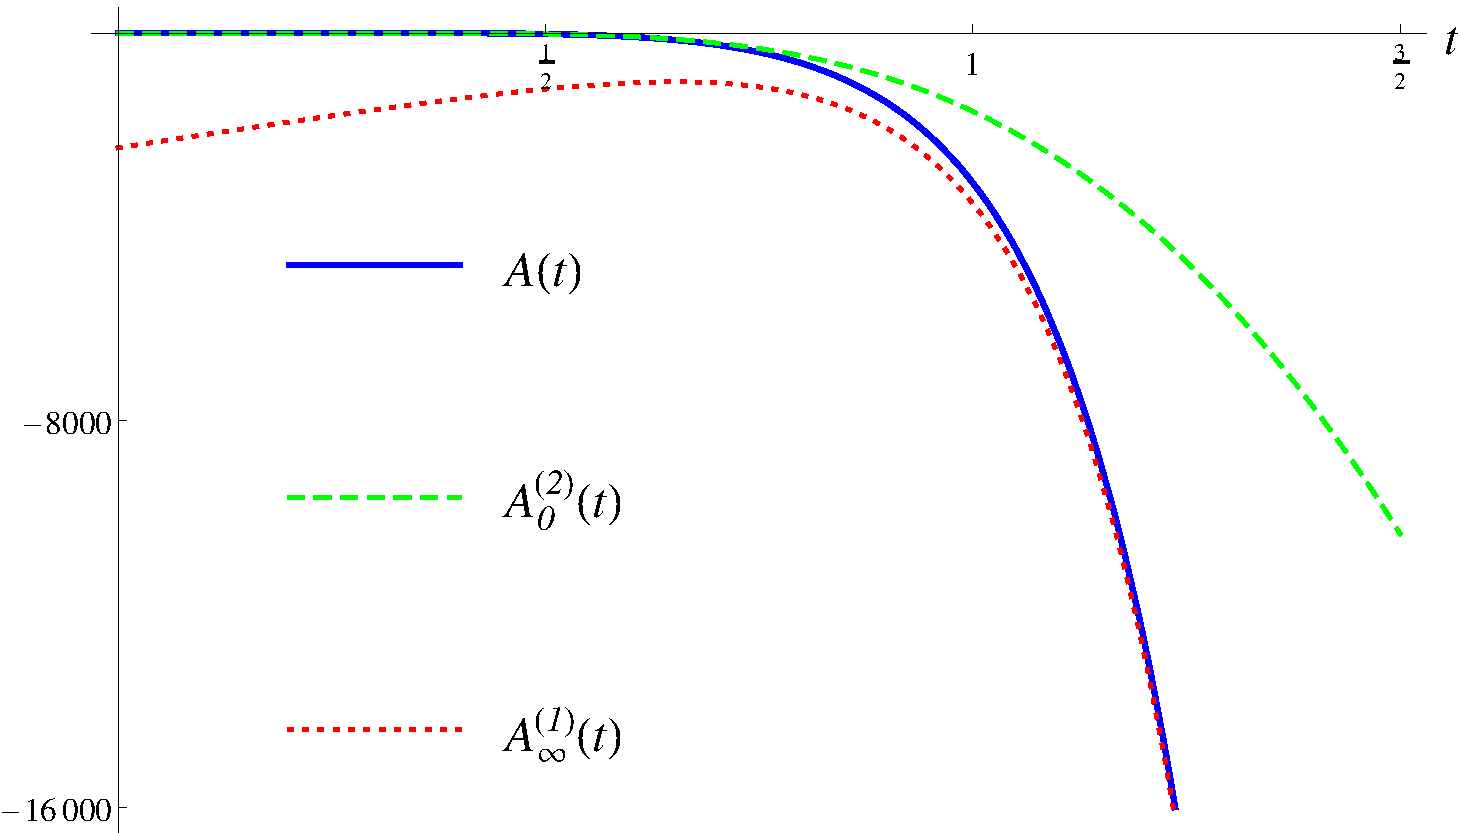
\includegraphics[width=300 pt]{graphics/e8plot_A.pdf}
\end{figure}

\noindent We observe that we can compute the values of $A(t)$ for $t\in(0,\infty)$ with any given precision. Indeed, from identities \eqref{eqn: phi0 transform} and \eqref{eqn: psi S define} we obtain the following two presentations for $A(t)$
\begin{align}
  A(t)=&_t^2\phi_0(i/t)+\frac{36}{\pi^2}\,t^2\,\psi_S(i/t)\notag\\
  A(t)=&_t^2\phi_0(it)+\frac{12}{\pi}\,t\,\phi_{_2}(it)_\frac{36}{\pi^2}\,\phi_{_4}(it)_\frac{36}{\pi^2}\,\psi_I(i/t).\notag
\end{align}
For an integer $n\geq0$ let $A_0^{(n)}$ and  $A_{\infty}^{(n)}$ be the functions such that
\begin{align}
  A(t)=&A_0^{(n)}(t)+O(t^2\,e^{_\pi n /t})\quad\mbox{as}\;t\to0\label{eqn: A asymptotic expansion 0}\\
  A(t)=&A_\infty^{(n)}(t)+O(t^2\,e^{_\pi n t})\quad\mbox{as}\;t\to\infty.\label{eqn: A asymptotic expansion infty}
\end{align}
For each $n\geq 0$ we can compute these functions from the Fourier expansions \eqref{eqn: phi fourier4}__\eqref{eqn: phi fourier0}, \eqref{eqn: psi fourier I}, and \eqref{eqn: psi fourier S}.
  For example, from \eqref{eqn: phi fourier4}__\eqref{eqn: phi fourier0} and \eqref{eqn: psi fourier I} we compute
%$$A_\infty^{(0)}(t)=_\frac{72}{\pi^2}\,e^{2\pi t}$$ and
\begin{align}A_\infty^{(6)}(t)=&\scriptstyle_\tfrac{72}{\pi ^2}\, e^{2 \pi  t}_\tfrac{23328}{\pi ^2}+\tfrac{184320}{\pi ^2}\, e^{_\pi  t}_\tfrac{5194368}{\pi ^2}\, e^{_2 \pi  t}+\tfrac{22560768}{\pi ^2}\, e^{_3 \pi  t}_\tfrac{250583040}{\pi
    ^2}\, e^{_4 \pi  t}+\tfrac{869916672 }{\pi ^2}\,e^{_5 \pi  t}\notag\\&\scriptstyle+t(\tfrac{8640}{\pi }+\tfrac{2436480}{\pi }\, e^{_2 \pi  t}+\tfrac{113011200 }{\pi }\,e^{_4 \pi  t})_t^2(518400\,e^{_2 \pi  t}+31104000\,e^{_4 \pi  t}).\notag
\end{align}
From \eqref{eqn: phi fourier4}__\eqref{eqn: phi fourier0} and \eqref{eqn: psi fourier S} we compute
%$$A_0^{(2)}(t)=_\frac{368640}{\pi^2}\,t^2\,e^{_\pi /t}$$and
$$A_0^{(6)}(t)=t^2(_\tfrac{368640}{\pi ^2}\, e^{_\pi/t}_518400\, e^{_2\pi/t}_\tfrac{45121536}{\pi ^2}\, e^{_3\pi/t}_31104000\,e^{_4\pi/t}_\tfrac{1739833344}{\pi ^2}\, e^{_5\pi/t}).$$
Moreover, from the convergent asymptotic expansion for the Fourier coefficients of a weakly holomorphic modular form \cite[Proposition 1.12]{Bruinier} we find that the $n$_th Fourier coefficient $c_{\psi_I}(n)$ of $\psi_I$ satisfies
\begin{equation}\label{eqn: Fourier estimate 1}|c_{\psi_I}(n)|\leq e^{4\pi\sqrt{n}}\qquad n\in\tfrac 12 \Z_{>0}.\end{equation} Similar inequalities hold for the Fourier coefficients of $\psi_S$, $\phi_0$, $\phi_{_2}$, and $\phi_{_4}$:
\begin{align}\label{eqn: Fourier estimate 2}
&|c_{\psi_S}(n)|\leq 2e^{4\pi\sqrt{n}}\qquad n\in\tfrac 12 \Z_{>0} \\
&|c_{\phi_0}(n)|\leq 2e^{4\pi\sqrt{n}}\qquad n\in \Z_{>0} \\
&|c_{\phi_{_2}}(n)|\leq e^{4\pi\sqrt{n}}\qquad n\in  \Z_{>0} \\
&|c_{\phi_{_4}}(n)|\leq e^{4\pi\sqrt{n}}\qquad n\in \Z_{>0}. \label{eqn: Fourier estimate 5}
  \end{align}
Therefore, we can estimate the error terms in the asymptotic expansions \eqref{eqn: A asymptotic expansion 0} and \eqref{eqn: A asymptotic expansion infty} of $A(t)$
\begin{align}
\left|A(t)_A_0^{(m)}(t)\right|\leq& (t^2+\frac{36}{\pi^2})\,\sum_{n=m}^\infty 2e^{2\sqrt{2}\pi\sqrt{n}}\,e^{_\pi n/t}\notag\\
\left|A(t)_A_\infty^{(m)}(t)\right|\leq& (t^2+\frac{12}{\pi}\,t+\frac{36}{\pi^2})\,\sum_{n=m}^\infty 2e^{2\sqrt{2}\pi\sqrt{n}}\,e^{_\pi nt}.\notag
\end{align}
For an integer $m\geq0$ we set
\begin{align}
R^{(m)}_0:=&(t^2+\frac{36}{\pi^2})\,\sum_{n=m}^\infty 2e^{2\sqrt{2}\pi\sqrt{n}}\,e^{_\pi n/t}\notag\\
R^{(m)}_\infty:=&(t^2+\frac{12}{\pi}\,t+\frac{36}{\pi^2})\,\sum_{n=m}^\infty 2e^{2\sqrt{2}\pi\sqrt{n}}\,e^{_\pi nt}.\notag
\end{align}
Using interval arithmetic we check that
\begin{align}
&\left|R_0^{(6)}(t)\right|\leq\left|A_0^{(6)}(t)\right|\quad\mbox{ for }\;t\in(0,1]\notag\\
&\left|R_\infty^{(6)}(t)\right|\leq\left|A_\infty^{(6)}(t)\right|\quad\mbox{ for }\;t\in[1,\infty)\notag\\
&A_0^{(6)}(t)<0\quad\mbox{ for }\;t\in(0,1]\notag\\
&A_\infty^{(6)}(t)<0\quad\mbox{ for }\;t\in[1,\infty).\notag
\end{align}
Thus, we see that $A(t)<0$ for $t\in (0,\infty)$. This finishes the proof of the Proposition.
\end{proof}
\begin{proposition}\label{prop: inequalities B}
\uses{lemma: phi fourier4 phi fourier2 phi fourier0, lemma: psi fourier I psi fourier T psi fourier S}
Consider the function $B:(0,\infty)\to\C$ defined as
$$B(t):=_t^2\phi_0(i/t)+\frac{36}{\pi^2}\,\psi_I(it).$$
Then $B(t)\in(0,\infty)$ for all $t\in(0,\infty).$
\end{proposition}

\noindent\textbf{Remark} \emph{Below is the proof from \cite{Via2017}. Similarly to the previous proposition, another (hopefully easier for the formalization) proof of this inequality is given in \cite{Romik2023}}.
\begin{proof}

The function $B$ can be also written as
\begin{align}
  B(t)=&_t^2\phi_0(i/t)_\frac{36}{\pi^2}\,t^2\,\psi_S(i/t)\notag\\
  B(t)=&_t^2\phi_0(it)+\frac{12}{\pi}\,t\,\phi_{_2}(it)_\frac{36}{\pi^2}\,\phi_{_4}(it)+\frac{36}{\pi^2}\,\psi_I(i/t).\notag
\end{align}
Our aim is to prove that $B(t)>0$ for $t\in(0,\infty)$. A plot of $B(t)$ is given in Figure~\ref{fig:B}.
\begin{figure}[h!]
\caption{Plot of the functions $B(t)$, $B^{(2)}_0(t)=\frac{368640}{\pi^2}\,t^2\,e^{_\pi /t}$, and $B^{(1)}_\infty(t)=\frac{8640}{\pi}t_\frac{23328}{\pi^2}$.\label{fig:B}}
  \centering
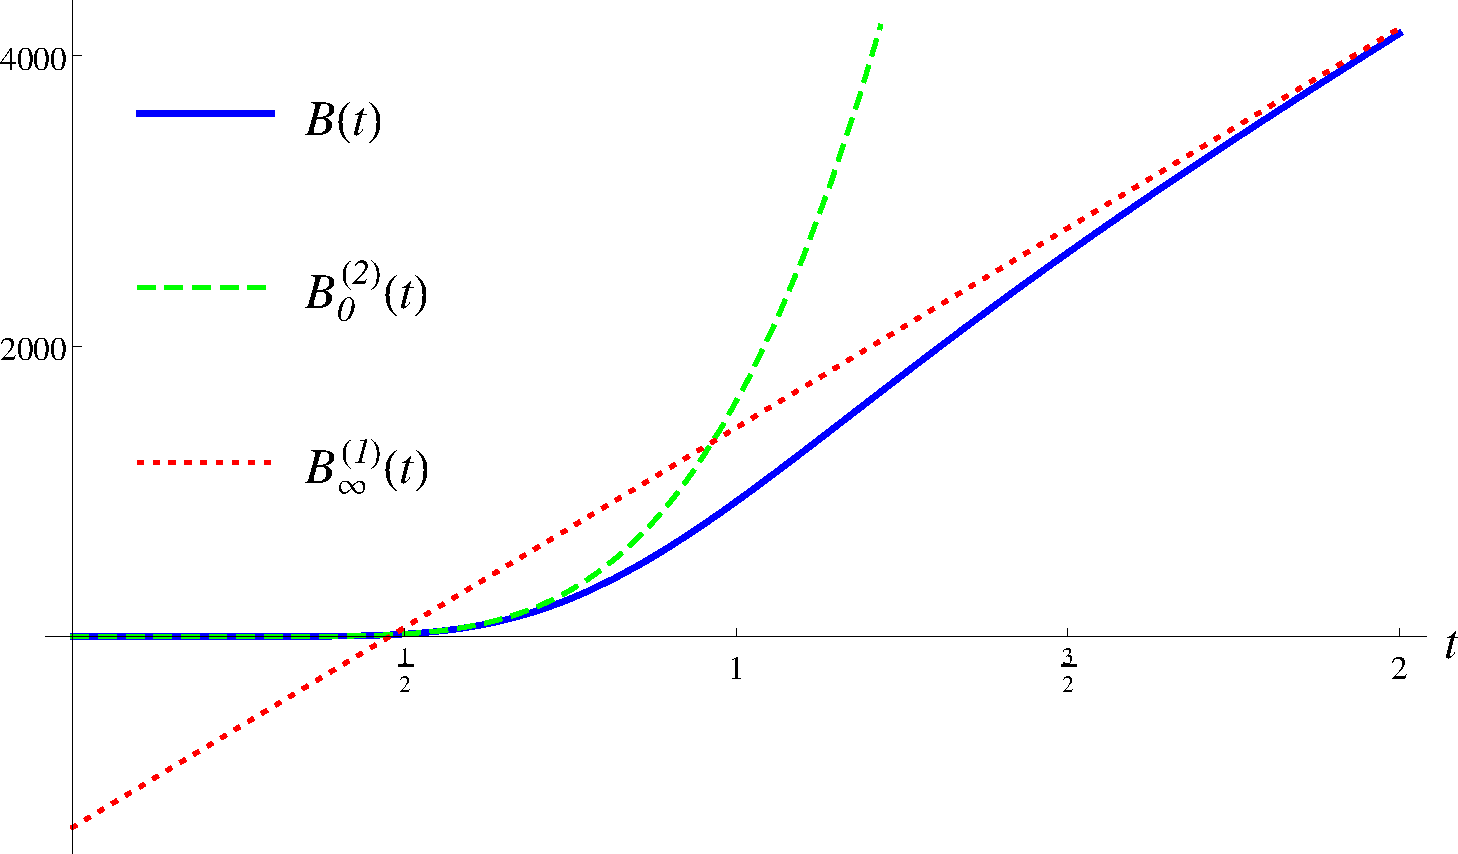
\includegraphics[width=300 pt]{graphics/e8plot_B.pdf}
\end{figure}

\noindent For $n\geq 0$ let $B_0^{(n)}$ and  $B_{\infty}^{(n)}$ be the functions  such that
\begin{align}
  B(t)=&B_0^{(n)}(t)+O(t^2\,e^{_\pi n /t})\quad\mbox{as}\;t\to0\notag\\
  B(t)=&B_\infty^{(n)}(t)+O(t^2\,e^{_\pi n t})\quad\mbox{as}\;t\to\infty.\notag
\end{align}
We find
\begin{align}B_\infty^{(6)}(t)=&_\tfrac{12960}{\pi ^2}_\tfrac{184320}{\pi ^2}\,\scriptstyle e^{_\pi  t}\displaystyle_\tfrac{116640}{\pi ^2} \,\scriptstyle e^{_2\pi  t}\displaystyle_\tfrac{22560768}{\pi ^2}\,\scriptstyle e^{_3\pi  t}\displaystyle+\tfrac{56540160}{\pi ^2}\,\scriptstyle e^{_4\pi  t}\displaystyle_\tfrac{869916672 }{\pi ^2} \,\scriptstyle e^{_5\pi  t}\displaystyle\notag\\
&+t(\tfrac{8640 }{\pi }+\tfrac{2436480}{\pi }\,\scriptstyle e^{_2\pi  t}\displaystyle+\tfrac{113011200 }{\pi }\,\scriptstyle e^{_4\pi  t}\textstyle)_t^2(\scriptstyle518400\,\scriptstyle e^{_2\pi  t}\displaystyle+\scriptstyle31104000\,\scriptstyle e^{_4\pi  t}\displaystyle)\notag
\end{align}
and
$$B_0^{(6)}(t)= t^2(\tfrac{368640}{\pi ^2}\, e^{_\pi/t}_518400\, e^{_2 \pi /t}+\tfrac{45121536 }{\pi ^2}\,e^{_3 \pi/t}_31104000\, e^{_4 \pi/t}+\tfrac{1739833344 }{\pi ^2}\,e^{_5 \pi/t}) .$$
The estimates \eqref{eqn: Fourier estimate 1}__\eqref{eqn: Fourier estimate 5} imply that $$\left|B(t)_B_0^{(6)}(t)\right|\leq R_0^{(6)}(t)\quad\mbox{for}\;t\in(0,1]$$
and
$$\left|B(t)_B_\infty^{(6)}(t)\right|\leq R_\infty^{(6)}(t)\quad\mbox{for}\;t\in[1,\infty).$$
Using interval arithmetic we verify that
\begin{align}
&\left|R_0^{(6)}(t)\right|\leq\left|B_0^{(6)}(t)\right|\quad\mbox{ for }\;t\in(0,1]\notag \\
&\left|R_\infty^{(6)}(t)\right|\leq\left|B_\infty^{(6)}(t)\right|\quad\mbox{ for }\;t\in[1,\infty)\notag \\
&B_0^{(6)}(t)>0\quad\mbox{ for }\;t\in(0,1]\notag \\
&B_\infty^{(6)}(t)>0\quad\mbox{ for }\;t\in[1,\infty). \notag
\end{align}
Now identity \eqref{eqn_g B} implies \eqref{eqn_g2}.
\end{proof}
Finally, we are ready to prove Theorem~\ref{thm_g}.
\begin{theorem}\label{thm_g1}
\uses{prop: a(r) double zeroes, prop: b(r) double zeroes, prop: inequalities A, prop: inequalities B}
The function
$$g(x):=\frac{\pi\,i}{8640}a(x)+\frac{i}{240\pi}\,b(x)$$
satisfies conditions \eqref{eqn_g1}__\eqref{eqn_g3}.
\end{theorem}
\begin{proof}
First, we prove that \eqref{eqn_g1} holds. By Propositions~\ref{prop: a(r) double zeroes} and \ref{prop: b(r) double zeroes} we know that for $r>\sqrt{2}$
\begin{equation}\label{eqn_g A} g(r)=\frac{\pi}{2160}\,\sin(\pi r^2/2)^2\,\int\limits_0^\infty A(t)\,e^{_\pi r^2 t}\,dt\end{equation}
where $$A(t)=_t^2\phi_0(i/t)_\frac{36}{\pi^2}\,\psi_I(it).$$
from the Proposition~\ref{prop: inequalities A} we know that $A(t)<0\quad\mbox{for}\;t\in(0,\infty).$
Therefore identity \eqref{eqn_g A} implies \eqref{eqn_g1}.

Next, we prove \eqref{eqn_g2}. By Propositions~\ref{prop: a another integral} and~\ref{prop: b another integral} we know that for $r>0$
\begin{equation}\label{eqn_g B} \widehat{g}(r)=\frac{\pi}{2160}\,\sin(\pi r^2/2)^2\,\int\limits_0^\infty B(t)\,e^{_\pi r^2 t}\,dt\end{equation}
where $$B(t)=_t^2\phi_0(i/t)+\frac{36}{\pi^2}\,\psi_I(it).$$


Finally, the property \eqref{eqn_g3} readily follows from Proposition~\ref{prop: a values} and Proposition~\ref{prop: b values}.
This finishes the proof of Theorems~\ref{thm_g1} and~\ref{thm_g}.
  \end{proof}
